%\chapterauthor{Author Name}{Author Affiliation}
%\chapterauthor{Second Author}{Second Author Affiliation}
\chapter{Brief Introduction to Linux}

This chapter gives a brief introduction to Linux, including its key features, advantages and disadvantages over other operating systems.

\section{Linux as an Operating System}

Linux is an \mync{Operating System}[OS]. An OS is essentially a special piece of software running on a machine (desktop, laptop, server, mobile devices, edge device, etc.) that manages hardware resources and supports application software in the system. An OS shall be able to:
\begin{itemize}
  \item Detect and prepare hardware.
  \item Manage process.
  \item Manage memory.
  \item Manage storage and files.
  \item Provide user and application interface, and associated authentication methods.
  \item Provide \myabb{software development kits}{SDK} for developing applications.
\end{itemize}

Linux has been overwhelmingly successful and adopted in many areas. For example, Android operating system for mobile phones is developed using Linux. Google Chrome is also backed by Linux. Many website such as Facebook are also running on Linux servers.

Some of the most favorable features of Linux, especially to large-size enterprises, are as follows.
\begin{itemize}
  \item Clustering. It is possible to group multiple Linux machines and let them work as a whole. The group of machines appears to be a single powerful machine to the upper layer.
  \item Visualization. It is possible to share a server among multiple users and applications in a logically separated manner, so that each of the users thinks that he is working on a dedicated machine.
  \item Cloud computing. Cloud computing is an advanced usage of Linux clustering and virtualization features. Linux servers can be configured flexibly to support cloud computing functions. It is convenient to manage and audit the users and the resources they deploy. 
  \item Real-time computing and edge computing. Embedded Linux can be implemented on micro-controllers or micro-computers for real-time edge control.
\end{itemize}
This list can go on and on.

Linux differs from Microsoft Windows and MacOS in many ways, though they are all very successful OSs. Among the three OSs, Linux is the only one that is completely open-source, in the sense that its source code can be viewed and customized by the users per requested.

\section{A Brief History of Linux}

The initial motivation of Linux is to create a UNIX-like operating system that can be freely distributed in the community.

Many modern OSs including MacOS and Linux are inspired by UNIX. UNIX operating system was created by AT\&T in 1969 as a software development environment that it used internally. In 1973, UNIX was rewritten in C language, thus gaining useful features such as portability. Today, C is still the primary language used to create UNIX and Linux kernels.

AT\&T, who originally owned UNIX, tried to make money from it. Back then AT\&T was restricted from selling computers per required by the government. Therefore, AT\&T decided to license UNIX source code to universities for a nominal fee. Researchers from universities started learning and improving UNIX, which speeded up the development of UNIX. In 1976, UNIX V6 became the first UNIX that was widely spread. UNIX V6 was developed at UC Berkeley and was named the \myabb{Berkeley Software Distribution}{BSD} of UNIX.

From then on, UNIX moved towards two separated directions. While BSD remained ``open'', AT\&T started steering UNIX towards commercialization. By 1984 AT\&T was pretty ready to start selling commercialized UNIX, namely ``AT\&T: \myabb{UNIX System Laboratories}{USL}''. USL did not sell very well. As AT\&T was not allowed to sell PCs, the only thing it could do was to license the source code to other PC manufactures. For this reason the price for the source code had to be set high as it was targeting PC manufactures, not end users. This effectively prevented an end user from procuring UNIX source code from AT\&T directly. The PC manufactures were more profitable than AT\&T just by selling UNIX-based PCs and workstations to the end users. Overall, although the community acknowledged that UNIX was useful, UNIX source code was extremely costly and was not popular among the end users.

In 1984, Richard Stallman started the GNU project as part of the Free Software Foundation. It is recursively named by phrase ``\myabb{GNU is Not UNIX}{GNU}'', intended to become a recording of the entire UNIX that could be open and freely distributed. The community started to ``recreate'' UNIX based on the defined interface protocols published by AT\&T.

Linus Trovalds started creating his version of UNIX, i.e. Linux, in 1991. He managed to publish the first version of the Linux kernel on August 25, 1991, which only worked on a 386 processor. Later in October, Linux 0.0.2 was released with many parts of the code rewritten in C language, making it more suitable for cross-platform usage. This Linux kernel was the last and the most important piece of code to complete a UNIX-like system under GNU General Public License (GPL). It is so important that people call this operating system ``Linux OS'' instead of ``GNU OS'', although GNU is the host of the project and Linux kernel is just a part (the most important part) of it.

\section{Linux Distributions}

As casual Linux users, people do not want to understand and compile the Linux source code to use Linux. In response to this need, different Linux distributions have emerged. They share the same Linux OS kernel but differ from each other in many ways such as software management tools and user interfaces.

Today, there are hundreds of Linux distributions in the community. The most famous two categories of distributions are as follows. The major difference is the way they manage software applications.
\begin{itemize}
  \item Red-Hat-Based Distributions
  \begin{itemize}
    \item \mync{Red Hat Enterprise Linux}[RHEL]
    \item Fedora
    \item CentOS
  \end{itemize}
  \item Debian-Based Distributions
  \begin{itemize}
    \item Debian
    \item Ubuntu
    \item Linux Mint
    \item Elementary OS
    \item Raspberry Pi OS
  \end{itemize}
\end{itemize}

Notice that although the source code of all the distributions above is publicly available as required by \myabb{GNU General Public License}{GPL} (GPL requires that any modified versions of a GPL-licensed product shall also be made open-source with a GPL license, as long as the modifications spread in the community), some of the distributions may come with a ``subscription fee''. The subscription fee is not for the OS source code, but for the technical support, paid maintenance, and other add-on services that the developers of the distributions provide to the end users.
 
\subsection{Red-Hat-Based Distributions}

Red Hat created the \mync{Red Hat Package Manager}[RPM] to manage software applications. The RPM packaging contains not only the software files but also its metadata, including version tracking, the creator, the configuration files, etc. In the OS, a local RPM database is used to track all software on the machine. \mync{Yellow Dog Updater Modified}[YUM] is an open-source Linux package management application that uses RPM plus additional features for enhanced user experience. YUM is very popular among Red-Hat-based distributions.

RHEL is a commercial, stable and well-supported OS that can host mission-critical applications for big business and governments. To use RHEL, customers pay for subscriptions which allow them to deploy any version of RHEL as desired. Different tiers of supports are available depending on the subscriptions. Many add-on features are available for the customers such as the cloud computing integration.

CentOS is a ``recreation'' version of RHEL using freely available RHEL source code. In this sense, CentOS experience should be very similar with RHEL and it is free of charge, but the users will not enjoy the professional technical support from RHEL engineers. Recently, Red Hat took over the development of CentOS project.

Fedora is a free, cutting-edge Linux distribution sponsored by Red Hat. It is less stable than RHEL, and plays as the ``testbed'' for Red Hat to interact with the community. From this perspective, Fedora is very similar to RHEL, just with more dynamics and uncertainties. Some functions, especially server related functions, will be tested on Fedora before implemented on RHEL.

\subsection{Debian-Based Distributions}

Different from Red-Hat-based distributions that use RPM, Debian and Debian-based distributions use \mync{Advanced Packaging Tool}[APT] to manage software applications. ATP simplifies the process of managing software by automating the retrieval, configuration and installation of software packages. Among all the Debian-based distributions, Ubuntu is the most successful and popular one. Ubuntu has a variety of graphical tools and focuses on full-featured desktop system while still offering popular server packages. It has a very active community to support its development.

Ubuntu has larger software pool than Fedora. Ubuntu and its associated software usually have a longer ``lifespan'' than Fedora because Ubuntu servers as a stable platform while Fedora is more of a ``testbed''. Ubuntu is more for casual users and beginners, while Fedora more for advanced users or developers, especially developers for RHEL.

\section{Linux Graphical Desktop}

Graphical user interface is not necessary to run Linux OS. Yet, many Linux distributions support graphical desktops to convene the end users. When installing these distributions, the user can choose whether or not to install a graphical desktop environment along with the OS. The most popular desktop environment is GNOME. There are other choices such as KDE, LXDE and Xfce desktops. GNOME and KDE are more for regular PCs while LXDE and Xfce, being light in size, more for low-power-demanding systems.

Figures \ref{ch:bitl:fig:gnomedemo}, \ref{ch:bitl:fig:kdedemo}, \ref{ch:bitl:fig:lxdedemo} and \ref{ch:bitl:fig:xfcedemo} give the flavors of each desktop environment mentioned above. From the figures we can see that GNOME adopts a more Linux/MacOS style desktop environment, while KDE ``Windows 7'' style. LXDE and Xfce are more simple in graphics presentations and they are more for embedded systems.

\begin{figure}[!htb]
	\centering
	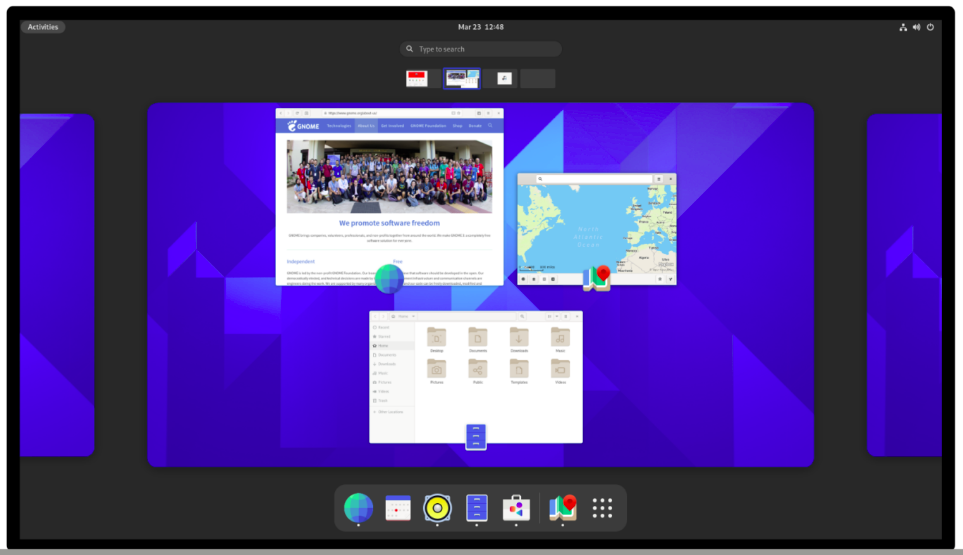
\includegraphics[width=250pt]{chapters/part-1/figures/gnome_demo.png}
	\caption{GNOME desktop environment.} \label{ch:bitl:fig:gnomedemo}
\end{figure}

\begin{figure}[!htb]
	\centering
	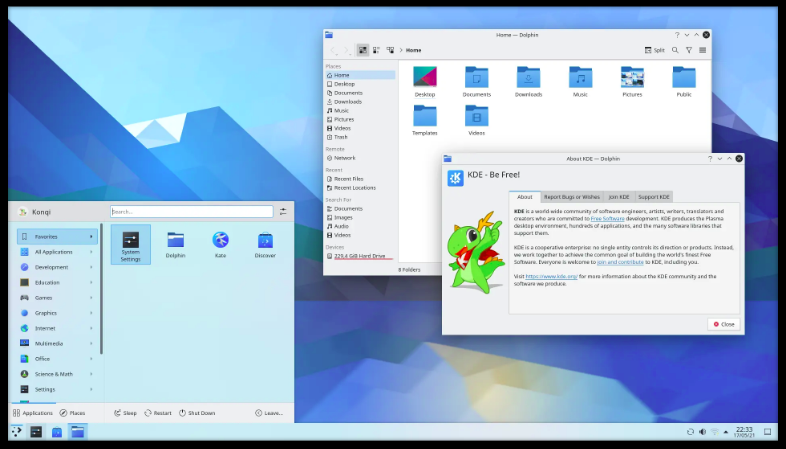
\includegraphics[width=250pt]{chapters/part-1/figures/kde_demo.png}
	\caption{KDE desktop environment.} \label{ch:bitl:fig:kdedemo}
\end{figure}

\begin{figure}[!htb]
	\centering
	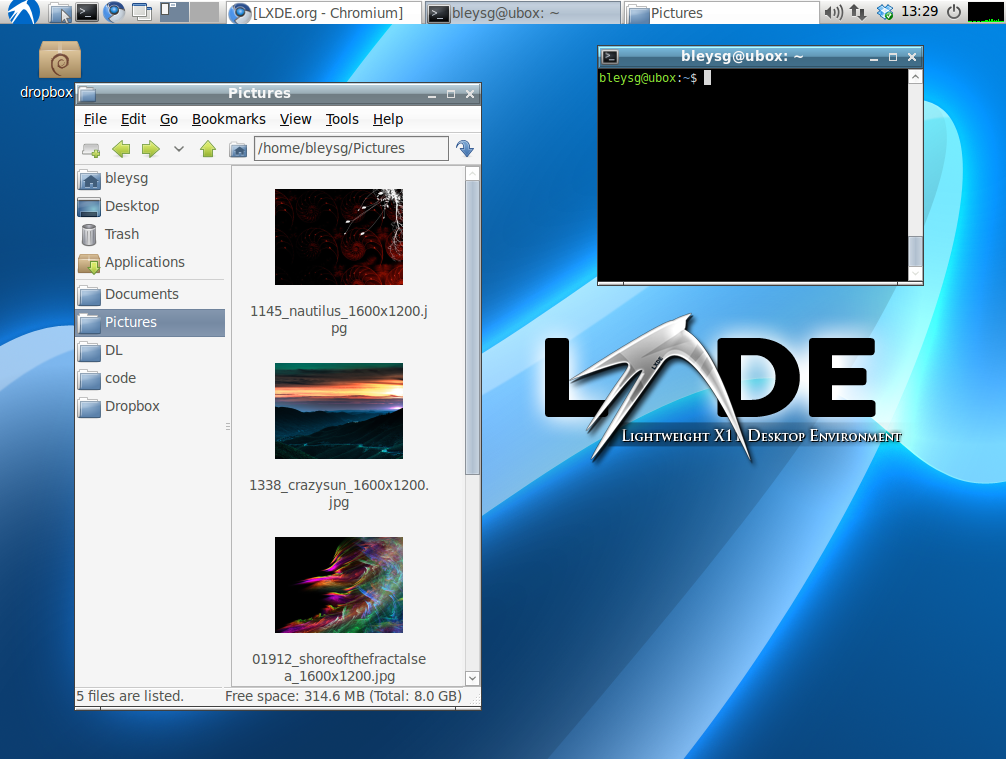
\includegraphics[width=250pt]{chapters/part-1/figures/lxde_demo.png}
	\caption{LXDE desktop environment.} \label{ch:bitl:fig:lxdedemo}
\end{figure}

\begin{figure}[!htb]
	\centering
	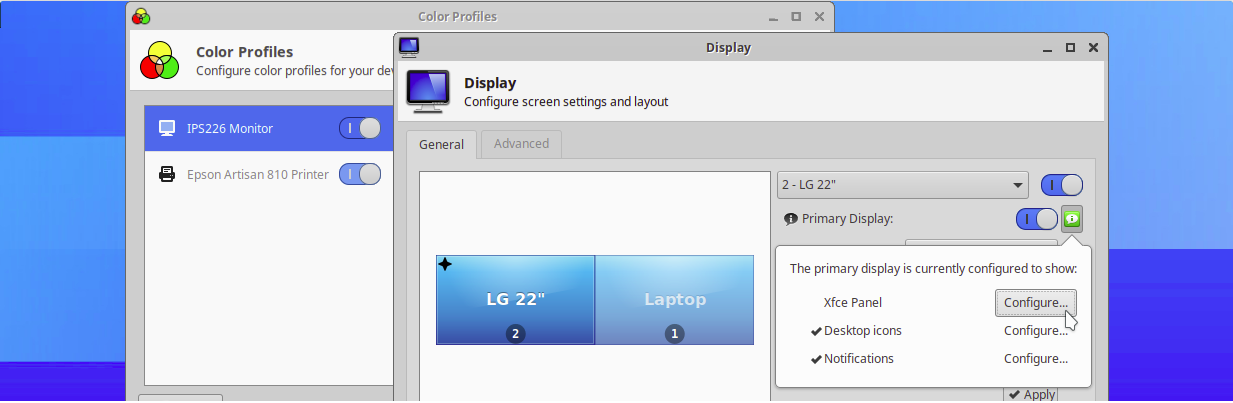
\includegraphics[width=250pt]{chapters/part-1/figures/xfce_demo.png}
	\caption{Xfce desktop environment.} \label{ch:bitl:fig:xfcedemo}
\end{figure}

It is possible to install multiple desktop environments on one machine, in which case the user can choose which desktop environment to use each time the computer is started.

\section{Linux Installation}

Linux can be installed both on a fixed hard drive or on a mobile storage such as a thumb drive. The installation of different distributions may differ. Thanks to the graphical installation tools for the popular distributions, the installations can be done fairly easily.

Instructions of installing Ubuntu is given by \textit{https://ubuntu.com}. Instructions of installing Fedora is given by \textit{https://getfedora.org}. For the use of RHEL, consult with Red Hat at \textit{https://www.redhat.com}. Red Hat provides different types of RHEL licenses for different using purpose, including developer license, which is cheaper than a standard enterprise-level license and serves well for learning purpose.
